% ---------------------------------------------------- %
% Budburst 2015 manuscript
% Preamble
% ---------------------------------------------------- %
\documentclass{article}
\usepackage{textcomp}
\usepackage{fontenc}
\usepackage{graphicx}
\usepackage{caption} % for figure captions
\usepackage{gensymb} % for \degree
\usepackage{placeins} % for \images
\usepackage[margin=1in]{geometry} % to set margins
\usepackage{setspace}
\usepackage{lineno}
\usepackage{cite}

\doublespacing
\renewcommand{\familydefault}{\sfdefault}
\graphicspath{{images/}}	% Root directory of the figures
\setlength{\parskip}{2 mm}

\usepackage{Sweave}
\begin{document}

\linenumbers
\Sconcordance{concordance:Budburst.tex:Budburst.Rnw:%
1 21 1 1 0 146 1 1 7 1 1 1 11 16 0 1 3 1 14 26 0 1 2 2 1 1 4 15 0 1 4 %
15 0 1 4 15 0 1 4 15 0 1 3 29 1}
 

\flushleft

\textbf{\large{Photoperiod and temperature interactively drive spring phenology in multiple species}}

Flynn, Wolkovich

\textit{The Arnold Arboretum of Harvard University}

%%%%%%%%%%%%%%%%%%%%%%%%%%%%%%%%%%%%
% Abstract
%%%%%%%%%%%%%%%%%%%%%%%%%%%%%%%%%%%%

\textbf{
% First two sentences are good -- but you only have room for one 'why to care about phenology' statement so adjust.
% Also need a quicker intro to design, including a clear problem statement. Consider something along the lines of: how diverse species respond to warming is a big question but few studies have looked at many species and such work has been generally observational. Observational studies, however, have known difficulties in teasing out plant responses to climate with are generally thought to be based on one or several major cues plant receive from the fall to spring: chilling temperatures, photoperiod and spring forcing temperatures. For a handful of well-studied temperate woody species these cues appear to be interactive, meaning predictions of plant responses to climate change will be complex and non-linear (cite CHUINE). Other work, however has suggested many species may be dominated by one of the three possible cues (cite Korner & Basler), making some species responses simple to predict. 
Woody plant spring phenology drives global carbon cycles and local ecosystem properties. Understanding the sensitivity of forest plants at the species level to abiotic drivers of plant phenology is critical for developing predictions of community composition, changes in community composition resulting from climate change, and resulting alterations to ecosystem-level properties such as carbon sequestration. While observational studies of long-term trends are essential for understanding how climate affects timing of phenological events, experimental manipulations are necessary to disentangle otherwise covarying environmental factors and directly assess species- and individual-level responses to climate change factors.
Here we present results from an experimental manipulation of spring forcing temperatures, photoperiod, and intensity of winter chilling with dormant clippings of 28 woody plant species from forest communities at two latitudes (42.5\degree N and 46\degree N). We show photoperiod sensitivity is common across northeastern woody plants and phenological sensitivity to photoperiod and temperature appears largely coordinated across species (i.e., species highly sensitive to temperature were also highly sensitive to photoperiod), with greater sensitivity of budburst and leafout to temperature than to photoperiod. Winter chilling exerts a large role in driving advances in spring phenology, for both budburst and leafout stages, yet surprisingly more intense chilling at 1.5\degree C resulted in less pronounced effects than at 4\degree C. Latitude of origin exerted surprisingly small effects on sensitivity to abiotic factors in driving spring phenology, indicating that local adaptation---at least across 4\degree of latitude---may not necessarily constrain woody plant responses to climate change. Shrub and small tree species were less sensitive to changing temperatures or photoperiod, but consistently earlier in their phenology. These results indicate that under warming conditions, communities could shift to a more canopy-tree dominated system.
}

%%%%%%%%%%%%%%%%%%%%%%%%%%%%%%%%%%%%
%Introduction 
%%%%%%%%%%%%%%%%%%%%%%%%%%%%%%%%%%%%

Woody plant spring phenology drives global carbon cycles and local ecosystem properties. Understanding the sensitivity of forest plants at the species level to abiotic drivers of plant phenology is thus critical for developing predictions of community and ecosystem-level properties. 

While observational studies of long-term trends are essential for understanding how climate affects timing of phenological events, experimental manipulations can disentangle otherwise covarying environmental factors and directly assess species- and individual-level responses to climate change factors. Early phenological events such as bud swelling and budburst are challenging to study from remote sensing, requiring experimental work at the individual level.

Timing of spring phenology is critical for understanding net ecosystem assimilation at the forest scale, as maximizing the length of the growing season and minimizing risk of tissue loss due to early spring freezing depends on accurate timing of budburst and leafout. 
\cite{Basler:2014aa}

Here we ask the following questions:
\begin{itemize}
\item{For a community of northeastern woody plants, what is the role of photoperiod versus temperature in determining timing of budburst, leaf-out, and flowering? Are species limited by photoperiod requirements in their response to warming temperatures? How consistent are such responses within communities?}
\item{To what extent do winter chilling requirements act as additional conservative strategy to avoid damage from early spring freezing?}
% What do you mean by this? 
\item{Do populations at northern sites, with more severe winters and shorter winter daylength, exhibit more conservative phenological strategies?}
% Need to define "conservative phenological strategies".
\end{itemize}

% I think we probably need to set up the hypotheses for plant strategies here more. I know I suggested the one about risk avoidance across sites that for that we *really need* to show that there is an increased risk of spring frost after leafout (or after some critical climate threshold) at one site versus the other. Otherwise it's unclear to me why one site would actually be 'riskier.' Certainly SH probably has a shorter growing season but I am no longer sure it's a riskier season climatically.
% On the other hand I think we should definitely set up more about risky or conservative strategies ACROSS the growing season. It would be easy to suggest that early species are 'riskier' and later species more conservative with regards to late frosts. I think we can also tie that into Koerner and Basler (but we should re-read it) and say that later a more photoperiod dominating cue system could be best.  
% This might also be a way to sneak in the traits possibly ... because I think the strategy could be early, risky but cheaper, less competitively dominant versus later, safer and more competitively dominant. Then the traits work provides a very simple test of this? And we say 'ah, teasing out the traits will be trickier and probably involve understanding which traits really tie to competitive superiority versus which might tie to frost resistance etc.. 

Photoperiod has long been known to be a critical driver of the onset of endormancy, in combination with cooling temperatures \cite{Foley:2009aa}. However, the role of photoperiod in determining the breadking of dormancy has been debated, with various authors finding that the strength of daylength as a driver may depend on phenological stage, species and location (Heide 1993; Kramer 1994; \cite{Falusi:1996aa}. Photoperiod and winter chilling can interact, as long as photoperiod enhances cell growth, compensating for a lack of chilling during the endodormancy phase (Chuine 2013; Wareing 1953; Heide 1993b.. \cite{Caffarra:2011aa} \cite{Myking:1995aa}. In the few experimental studies that have directly manipulated both forcing temperature and photoperiod, photoperiod has been shown to 

% The below is good but can probably move to the supplement and you can have just a sentence here saying 'A literature review (see Supp) shows that the most species examined for photoperiod and temperature cues in a manipulative study to date is four' or something like that. 
We conducted a literature review, finding 109 studies which investigated effects of photoperiod, temperature, or their interaction on the timing of bud burst or flowering for woody or semi-woody plants.  No study varied chilling period, photoperiod, and temperature simultaneously across multiple species at multiple sites. Of those studies, eight simultaneously manipulated photoperiod and temperature. Basler \& Koerner 14 found a negative tradeoff between sensitivity to photoperiod and sensitivity to warming for four species, for example with Fagus sylvatica advanced on average in leafout by 12 days in response to experimentally lengthened photoperiod, but only ca. 8 days in response to warmer temperatures, while Acer pseudoplatanus advanced in leafout by 17 days in response to warming but essentially had no change in response to photoperiod. The current study expands on this work by including 28 species, across two sites, with addition manipulations of chilling temperature.

Different phenological stages may be driven by different environmental cues. The period between budburst and leafout is critical for leaf development, as this is a period when plants are highly sensitive to damage from early frosts. Thus we carried out our tests for both budburst and leafout. We predicted that budburst would be generally less predictable than leafout. % Because ...



%%%%%%%%%%%%%%%%%%%%%%%%%%%%%%%%%%%%
\section*{Results}
%%%%%%%%%%%%%%%%%%%%%%%%%%%%%%%%%%%%

Temperature and photoperiod individually and interactively determined timing of leaf-out, with the strongest effects of temperature in short-day conditions. We found photoperiod sensitivity was common and strong across all of the woody plants studies, consistently reducing time to phenological responses for each species, across sites of origin. 

For the 28 species studied, sensitivity to temperature and photoperiod cues for leaf-out times varied substantially, and---in contrast to our hypotheses [that we set up in the intro]---co-varied overall. The coordinated response to warming temperatures and longer photoperiod was consistent with overall pace of phenological events; earlier-leafing out species (namely the shrubs \emph{Spiraea alba}, \emph{Viburnum cassanoides}, and \emph{Vaccinium myrtilloides}) exhibited relatively limited advances to either warming or longer days, while later leafing-out species showed ability to advance their phenology by in response to both warming and longer days. Thus, no trade-off was observed between photoperiod-cued and temperature-cued species, but rather species exhibit coordinated responses to both environmental factors (Fig. 1). Of the other species, \emph{Fagus grandifolia} exhibits relatively limited response to warming but substantial photoperiod sensitivity, while \emph{Rhamnus frangula} shows relatively limited response to photoperiod but substantial warming sensitivity; if only a small subset of species including these two had been included in the study, it might have been concluded that a tradeoff between photoperiod sensitivity and warming sensitivity would exist. % Nice!

While both photoperiod and temperature cues were important for driving woody plant phenology, responses to chilling were also substantial. Budburst day was accelerated most by the chilling treatments. Tables 1 and 2 summarizes hierarchical mixed-effects model analysis of day of budburst and leaf-out, with negative values indicate earlier day of experiment for each event. Overall the 5\degree C experimental warming resulted in 6.8 days earlier budburst and 21.9 days earlier leafout. Such advance was delayed by the each chilling treatment, as indicated by the positive coefficient for the temperature x chilling interactions. Latitude of origin (Site) overall had little direct effect on budburst or leaf-out, but populations from the northern site tended to exhibit slower budburst and leaf-out, with a more rapid budburst and leafout in response to the chilling treatments (indicated by negative coefficients for site x chilling treatments).

Warming, photoperiod, and chilling individually and interactively acted to drive budburst and leafout earlier across species. The strength of the acceleration in budburst due to both warming and photoperiod were similar, but the acceleration of leafout due to warming exceeded that of photoperiod for both phenological stages. Surprisingly, site of origin exerted limited effect on either budburst or leafout across species. 

\subsection*{Effect of chilling}
The cuttings were harvested in late January 2015, and thus experienced substantial natural chilling by the time they were harvested. Using weather station data from the Harvard Forest and St. Hippolyte site, chilling hours (below 7.2\degree C), Utah Model chill portions (hours below 7.2\degree C and between 0\degree C and 7.2\degree C) and Dynamic Model chill portions (Erez \& Fishman 1997) were calculated both for the natural chilling experienced by harvest and the chilling experienced in the 4\degree C and 1.5\degree C treatments. With both the Utah and Dynamic model, the more severe chilling treatment resulted in fewer calculated chilling portions. % Need to describe each model super briefly!

Species varied widely in response to chilling treatments, with some exhibiting strong chilling requirements (\emph{Acer saccharum}, \emph{Fagus grandifolia}), while others exhibited little change in phenological advancement under experimentally manipulated chilling. Overall, budburst and leaf-out advanced by 22.1 or 26.4 days under additional 30 d of vernalization at 4\degree C, and advanced by a reduced amount of 19.7 or 26.1 days under 30 d of vernalization at 1.5\degree C. The reduced chilling effect at the lower temperature chilling is consistent with the Dynamic Model of chilling accumulation. % And also consistent with the Utah model?

Species-specific responses to chilling demonstrate that chilling requirements are not uniform across species, with 
of \emph{Fagus grandifolia} to increasingly strong vernalization varies by latitude of origin and by phenological stage; winter chilling reduced day to budburst and leaf-out, but more strongly for individuals from the northern site.

While nearly all species showed advances in spring phenology in response to the experimental chilling treatment, as indicated by fewer days to phenological events for the 4\degree C and 1.5\degree C treatments, the majority of species (e.g. \emph{Populus grandidentata}) showed delays in both budburst and leafout at the more severe chilling treatment. Of the species exposed to the additional chilling, only \emph{Fagus grandifolia} was consistently advanced by the more severe chilling.

\subsection*{Species-specific responses}

Species traits partly explain variation in warming and photoperiod sensitivities of leafout. 
Plants with high nitrogen leaves, as well as high SLA (thinner, less dense) leaves, were significantly later in both budburst and leafout. Thus early leafout species tended to be tougher, less N-dense, and have higher carbon investments than later species. Greater wood density had inconsitent effects as a driver, with higher wood density driving later budburst but tending to drive earlier leafout.

Ring-porous species (\emph{Fraxinus sp.}, \emph{Lonicera}, \emph{Myrica}, and \emph{Quercus}; lower values of Pore Anatomy variable) exhibited significantly later budburst and leafout compared to diffuse-porous species, in line with previous work on wood anatomy and freezing risk (Sperrry \& Sullivan 1991 Plant Phys).

\subsection*{Nonleafouts}

Separate analysis of samples which did not break bud or leafout. Across species, there was no overall predictive effect of temperature, photoperiod, chilling, or site on the propensity to fail to leaf out. 
Species ranged from complete leafout (\emph{Hamamelis}) to only 50\% leafout (\emph{Fagus grandifolia}, \emph{Acer saccharum}) across all treatments. The percent of nonleafouts by site was similar, with 12.4\% of Harvard Forest and 9.5\% of St. Hippolyte samples failing to leaf out. Examining individual species,  there was an interaction of temperature by daylength for some species, with greater failure to leafout in cool, short conditions for \emph{Acer pensylvanicum}  and \emph{Acer saccharum}. Site effects were inconsistent, with greater failure to leafout for cuttings from St. Hippolyte in \emph{Acer rubrum} and \emph{Fagus grandifolia}, and from Harvard Forest in \emph{Acer saccharum}.

% I think you can cut the below
% All species show advances in budburst and leafout in response to photoperiod, warming, and chilling treatments. All species showed positive interactions between warming and chilling for leafout. For budburst, interactions between warming and chilling were always positive but not those between photoperiod and chilling (4 and 12 species showing positive interaction for chill1 and chill2, respectively).

Rank order of leafout and budburst was stable across warming and photoperiod treatments. Chilling treatments shifted the order, for example \emph{Fagus grandifolia} was always the 23-28th species to burst bud in chill0, but always the 10-11th species to burst bud in chiill1 and chill2. Within chilling treatments, the standard deviation of the rank order ranged from 2.05 (budburst, chill0) to 0.75 (leafout, chill1). 

%%%%%%%%%%%%%%%%%%%%%%%%%%%%%%%%%%%%
\section*{Discussion}
%%%%%%%%%%%%%%%%%%%%%%%%%%%%%%%%%%%%

\begin{itemize}

\item{Photoperiod sensitivity is common in northeastern woody plants; Phenological sensitivity to photoperiod and temperature are largely coordinated across species.}
\item{Chilling is the most important factor, even of greater importance than forcing. Mild winters spur greater phenological advancement than colder winters. Chilling much more important than temperature or photoperiod in driving earler budbreak, and still relatively more important for leafout. Chilling and forcing temperature are more substitutable than chilling and photoperiod, for both budburst and leafout.}
\item{Only limited support for risk-avoidance strategies for northern populations of these 28 species was found, with small delays in both phenological events for populations from the more northern site. The latitudinal range studied here is within the range of the phenotypic flexibility of these species. Of these study species, we should not be overly concerned about being photoperiod limited at the more northern sites; given sufficient pace of dispersal, they will be able to track a changing climate.}
\item{Budburst is sensitive to the same environmental cues as leafout, but species show idiosyncratic orderings of their sensitivity to environmental cues at these two phenological stages; leafout responses can not necessarily be used to back-cast budburst responses. Budburst showed a more limited total response to environmental cues, and species were more tightly clustered in those repsonses.}
\item{Surprisingly, the smaller statured, earlier-leafing out shrubs and small trees exhibited reduced sensitivity to all three factors of temperature, photoperiod, and chilling. They are relatively more fixed in their timing of both budburst and leafout, perhaps indicating an alternative mechaism for timing of spring phenology in these plants, such depending on carbohydrate metabolism to time budburst (Pagter 2015).}
\item{Given these results, the future of the northeastern forests may shift away from shrubs and small trees, as late-successional, later-event species demonstrated a greater ability to lengthen their growing seasons opportunistically in response to warmer temperatures.} % I think we should be more cautious in stating this. We still don't know *what* controls their leafout!
\end{itemize}

% Re the above about shrubs versus trees -- I am just not sure what to think! And it comes back to the models. Our models give each species a fundamental leafout day -- their intercept. This makes lots of sense to me but biologically I am not sure what to do with it (and if we take it away then the early species become hyper-sensitive, right?). I think we need to think on what that intercept means and what we should and shouldn't say given that it's in our models. I think it could be what you suggested, it could also be that they have super weak chilling, it could be that they are sensitive to humidity or something we don't study. But fundamentally I think we need to think harder about that before we push our conclusions too far. To discuss next week! And maybe we can ask people at the Stan meeting next Wednesday night. 

%%%%%%%%%%%%%%%%%%%%%%%%%%%%%%%%%%%%
\section*{Methods}
%%%%%%%%%%%%%%%%%%%%%%%%%%%%%%%%%%%%

\textbf{Field sampling}

Woody plant cuttings were made in January 2015 for 28 species which occurred in both Harvard Forest (HF, 42.5\degree N, 72.2\degree W) and the Station de Biologie des Laurentides in St-Hippolyte, Quebec (SH, 45.9\degree N, 74.0\degree W). The typical late January temperatures are -3.4 and -22\degree C, respectively; daylength between these two sites differs by a maximum of 45 minutes. Weather station data from each field site was obtained for calculations of chilling units. 

Cuttings were grown in growth chambers at the Arnold Arboretum in Boston, MA, in distilled water, with water changed every 7-10 days. Cuttings of an individual tree were exposed to each of 12 experimental treatments in a fully-factorial design: 2 temperature (20\degree C / 10\degree C warm vs. 15\degree C / 5\degree C cool) x 2 photoperiod (12 vs. 8 h) x 3 chilling (zero,  33 d at 4\degree C, 33 d at 1.5\degree C) treatments. 

With 6 replicates of these species across 6 experimental treatments being monitored at 5-7 day intervals for over 3 months, we made over 17,500 individual phenological observations following a modified BBCH scale.

\textbf{Growth chamber experiment}
Cuttings were kept in Erlenmyer flasks with distilled water. Water was changed every 7-12 days, with the bases of cuttings re-cut each time under water to prevent callusing.

Phenology was assessed using a modified BBCH scale (Finn et al. 2011), with observations on each of the 2136 cuttings made every 2-3 days for the course of the 82-day experiment.

\textbf{Statistical analysis}

Linear mixed effects models in R, then stan.

%%%%%%%%%%%%%%%%%%%%%%%%%%%%%%%%%%%%
\section*{References Cited}
%%%%%%%%%%%%%%%%%%%%%%%%%%%%%%%%%%%%

\bibliography{/Users/danflynn/Dropbox/References/Bibrefs/danlib}
\bibliographystyle{naturemag}

%%%%%%%%%%%%%%%%%%%%%%%%%%%%%%%%%%%%
\section*{Figures and Tables}
%%%%%%%%%%%%%%%%%%%%%%%%%%%%%%%%%%%%
\listoftables

\listoffigures



% latex table generated in R 3.2.3 by xtable 1.7-4 package
% Mon May  9 08:01:11 2016
\begin{table}[ht]
\centering
\caption{Chill units in field and field and growth chamber conditions.} 
\begin{tabular}{llrrr}
  \hline
Site & Treatment & Chilling Hours & Utah Model & Chill portions \\ 
  \hline
Harvard Forest & Field chilling & 892 & 814.50 & 56.62 \\ 
   & 4.0 \degree C x 30 d & 2140 & 2062.50 & 94.06 \\ 
   & 1.5 \degree C x 30 d & 2140 & 1702.50 & 91.17 \\ 
  St. Hippolyte & Field chilling & 682 & 599.50 & 44.63 \\ 
   & 4.0 \degree C x 30 d & 1930 & 1847.50 & 82.06 \\ 
   & 1.5 \degree C x 30 d & 1930 & 1487.50 & 79.18 \\ 
   \hline
\end{tabular}
\end{table}
% latex table generated in R 3.2.3 by xtable 1.7-4 package
% Mon May  9 08:01:11 2016
\begin{table}[ht]
\centering
\caption{Phylogenetic signal in timing of budburst and leafout and species specific traits, as estimated in the caper package with simultaneous fitting of lambda.  Pore anatomy (ring- versus diffuse-porous species) was highly clustered phylogenetically, but no other trait examined demonstrated significant phylogenetic signal} 
\begin{tabular}{lr}
  \hline
Relationship & Lambda \\ 
  \hline
SLA - Temperature & 0.000 \\ 
  SLA - Photoperiod & 0.000 \\ 
  SLA - Chilling 4 \degree C & 0.000 \\ 
  SLA - Chilling 1.5 \degree C & 0.000 \\ 
  Wood Density - Temperature & 0.000 \\ 
  Wood Density - Photoperiod & 0.000 \\ 
  Wood Density - Chilling 4 \degree C & 0.000 \\ 
  Wood Density - Chilling 1.5 \degree C & 0.000 \\ 
  \% N - Temperature & 0.285 \\ 
  \% N - Photoperiod & 0.203 \\ 
  \% N - Chilling 4 \degree C & 0.127 \\ 
  \% N - Chilling 1.5 \degree C & 0.130 \\ 
  Pore anatomy - Temperature & 1.000 \\ 
  Pore anatomy - Photoperiod & 1.000 \\ 
  Pore anatomy - Chilling 4 \degree C & 1.000 \\ 
  Pore anatomy - Chilling 1.5 \degree C & 1.000 \\ 
   \hline
\end{tabular}
\end{table}

% Trait tables
% latex table generated in R 3.2.3 by xtable 1.7-4 package
% Mon May  9 08:01:11 2016
\begin{table}[ht]
\centering
\caption{Trees, budburst} 
\begin{tabular}{rrrrrrr}
  \hline
 & est & se & stat & p & lwr & upr \\ 
  \hline
Intercept & 29.45 & 0.37 & 78.70 & 0.00 & 28.72 & 30.19 \\ 
  Stem density & 2.16 & 0.48 & 4.47 & 0.00 & 1.21 & 3.11 \\ 
  SLA & 1.70 & 0.38 & 4.52 & 0.00 & 0.96 & 2.44 \\ 
  % N & 1.30 & 0.45 & 2.87 & 0.00 & 0.41 & 2.19 \\ 
  Pore anatomy & -4.81 & 0.37 & -12.89 & 0.00 & -5.55 & -4.08 \\ 
   \hline
\end{tabular}
\end{table}% latex table generated in R 3.2.3 by xtable 1.7-4 package
% Mon May  9 08:01:11 2016
\begin{table}[ht]
\centering
\caption{Trees, leafout} 
\begin{tabular}{rrrrrrr}
  \hline
 & est & se & stat & p & lwr & upr \\ 
  \hline
Intercept & 42.91 & 0.44 & 97.56 & 0.00 & 42.04 & 43.77 \\ 
  Stem density & -2.81 & 0.60 & -4.68 & 0.00 & -3.98 & -1.63 \\ 
  SLA & 2.07 & 0.44 & 4.74 & 0.00 & 1.21 & 2.92 \\ 
  % N & -0.97 & 0.55 & -1.77 & 0.08 & -2.05 & 0.11 \\ 
  Pore anatomy & -3.52 & 0.42 & -8.35 & 0.00 & -4.35 & -2.70 \\ 
   \hline
\end{tabular}
\end{table}% latex table generated in R 3.2.3 by xtable 1.7-4 package
% Mon May  9 08:01:11 2016
\begin{table}[ht]
\centering
\caption{Shrubs, budburst} 
\begin{tabular}{rrrrrrr}
  \hline
 & est & se & stat & p & lwr & upr \\ 
  \hline
Intercept & 23.76 & 0.53 & 45.07 & 0.00 & 22.72 & 24.79 \\ 
  Stem density & -4.59 & 0.79 & -5.84 & 0.00 & -6.13 & -3.04 \\ 
  SLA & 0.29 & 0.52 & 0.55 & 0.58 & -0.74 & 1.32 \\ 
  % N & 2.12 & 0.94 & 2.27 & 0.02 & 0.28 & 3.96 \\ 
  Pore anatomy & 1.58 & 1.27 & 1.25 & 0.21 & -0.91 & 4.07 \\ 
   \hline
\end{tabular}
\end{table}% latex table generated in R 3.2.3 by xtable 1.7-4 package
% Mon May  9 08:01:11 2016
\begin{table}[ht]
\centering
\caption{Shrubs, leafout} 
\begin{tabular}{rrrrrrr}
  \hline
 & est & se & stat & p & lwr & upr \\ 
  \hline
Intercept & 27.16 & 0.68 & 39.69 & 0.00 & 25.82 & 28.50 \\ 
  Stem density & 0.56 & 0.93 & 0.60 & 0.55 & -1.28 & 2.39 \\ 
  SLA & 2.32 & 0.57 & 4.06 & 0.00 & 1.20 & 3.45 \\ 
  % N & 3.04 & 1.11 & 2.75 & 0.01 & 0.87 & 5.21 \\ 
  Pore anatomy & -1.11 & 1.63 & -0.68 & 0.50 & -4.32 & 2.10 \\ 
   \hline
\end{tabular}
\end{table}
%%%%%%%%%%% Figures
% 1. Raw data plot

\begin{figure} % alternative for Fig 1
\begin{center}
\caption{Coordinated responses of 28 woody plant species to photoperiod and temperature cues for leafout. Color of circle reflect average leafout day across treatments, across sites of origin, while size of circle represents the total number of clippings in the experiment---this varies mainly based on whether the species was found at both sites and whether it was exposed to all three chilling treatments, see Supp X for more details.} % Changed legend, check that I did it correctly please! Also, is this the raw data or model fits or what?
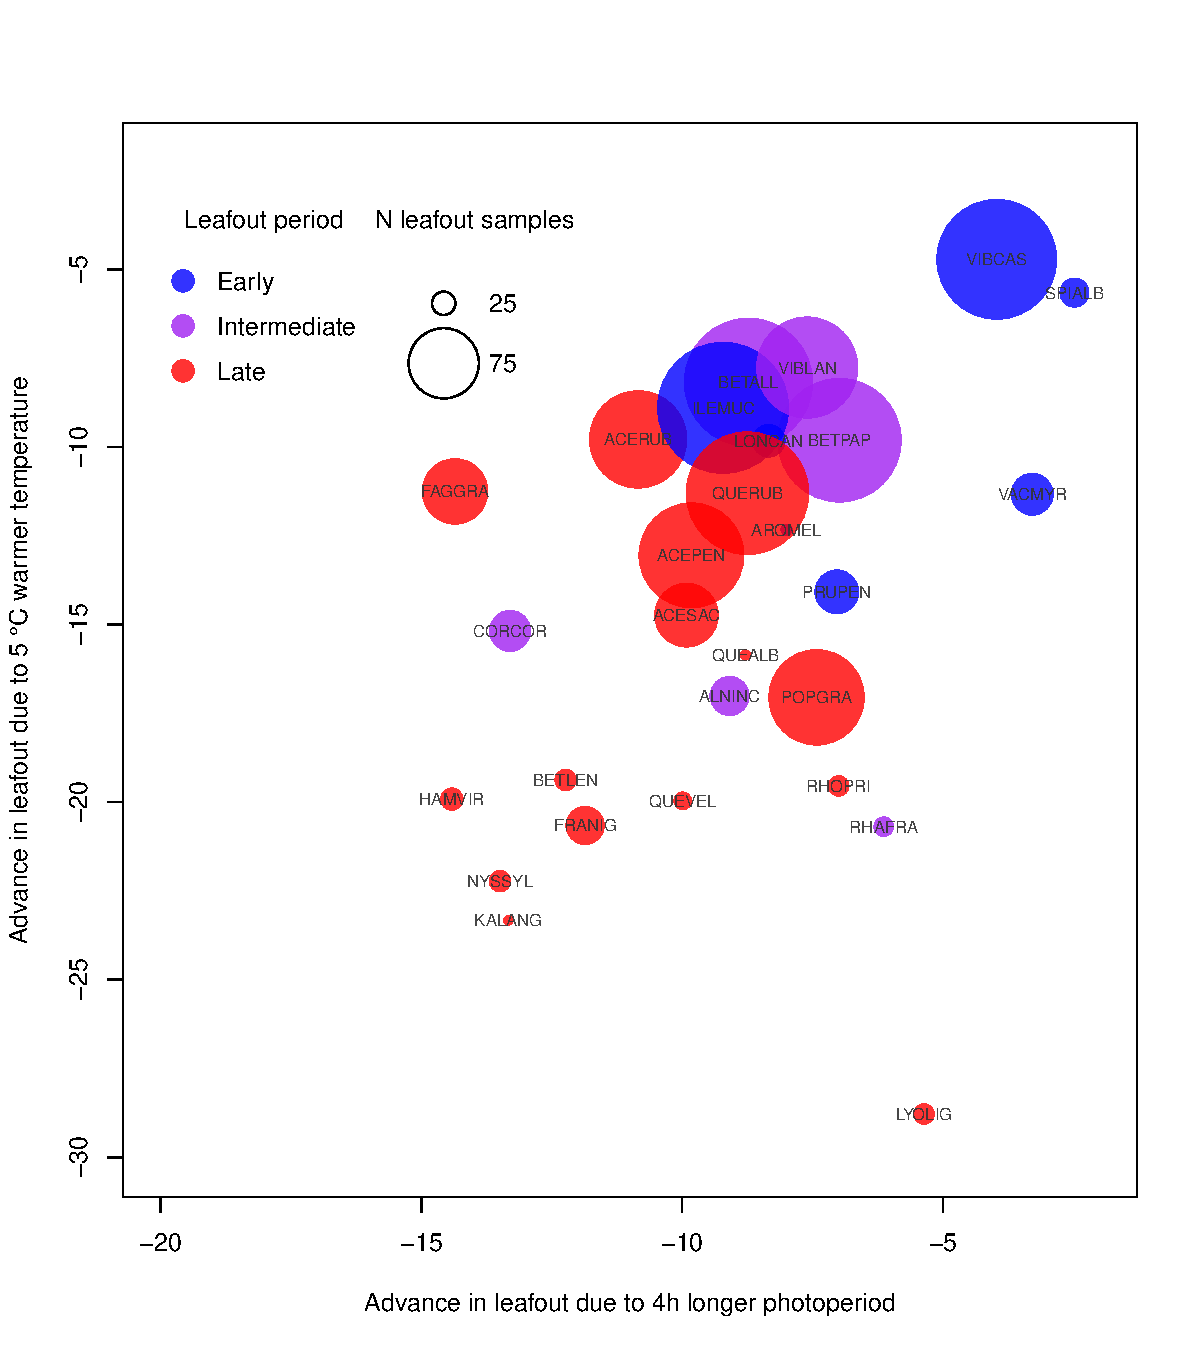
\includegraphics[scale=0.5]{Advplot2}
\label{fig1}
\end{center}
\end{figure}

% 2. model output
\begin{figure}
\begin{center}
\caption{Modeled effects plots, Budburst and Leafout}
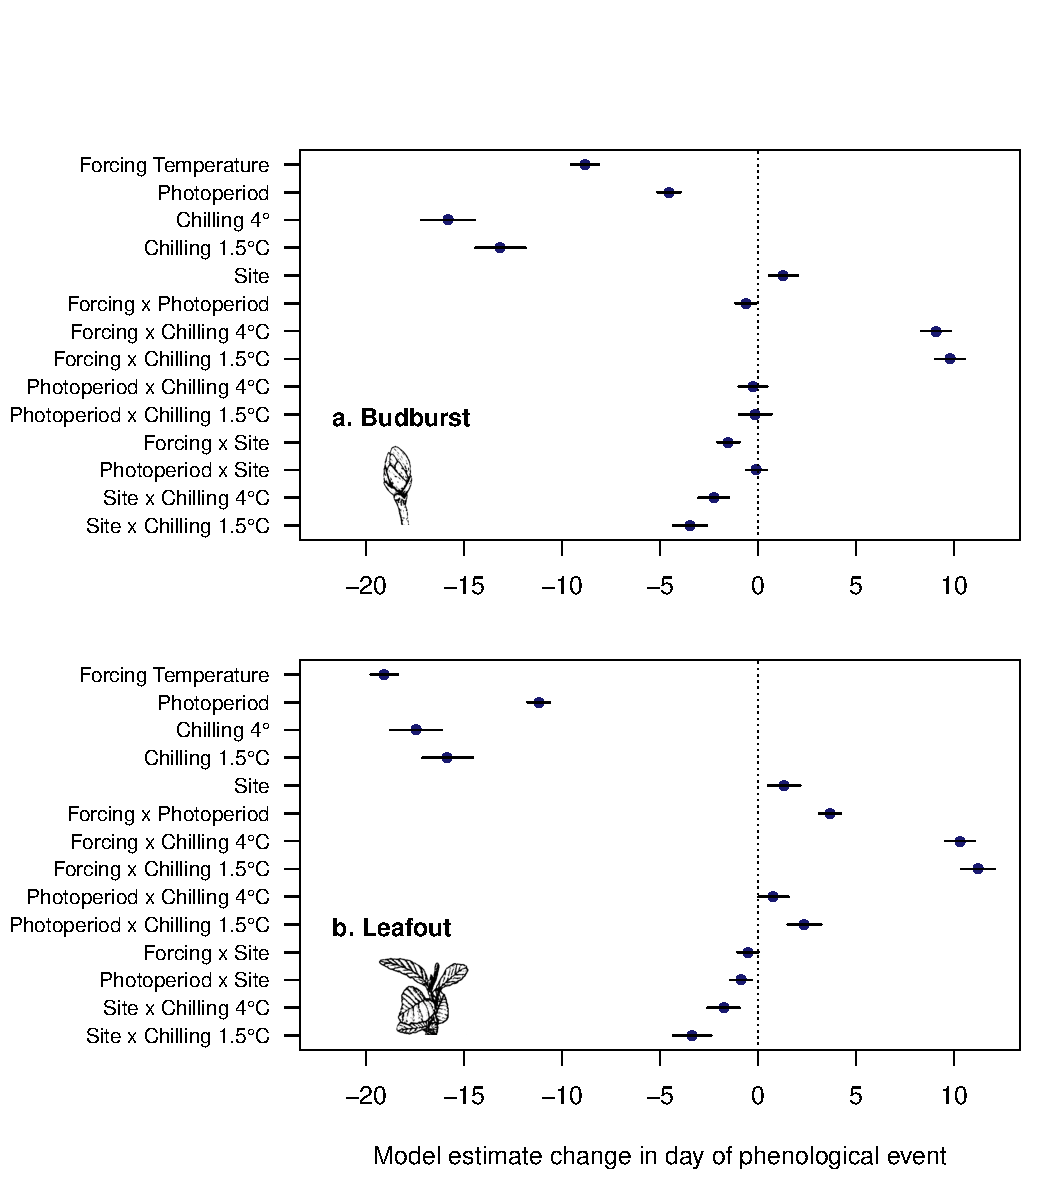
\includegraphics[scale=0.8]{Fig1_bb_lo}
\label{fig2}
\end{center}
\end{figure}

% 3. Temp + Pheno + Chill sensitivity

\begin{figure}
\caption{Sensitivity of budburst and leafout to warming, leafout, and chilling.}
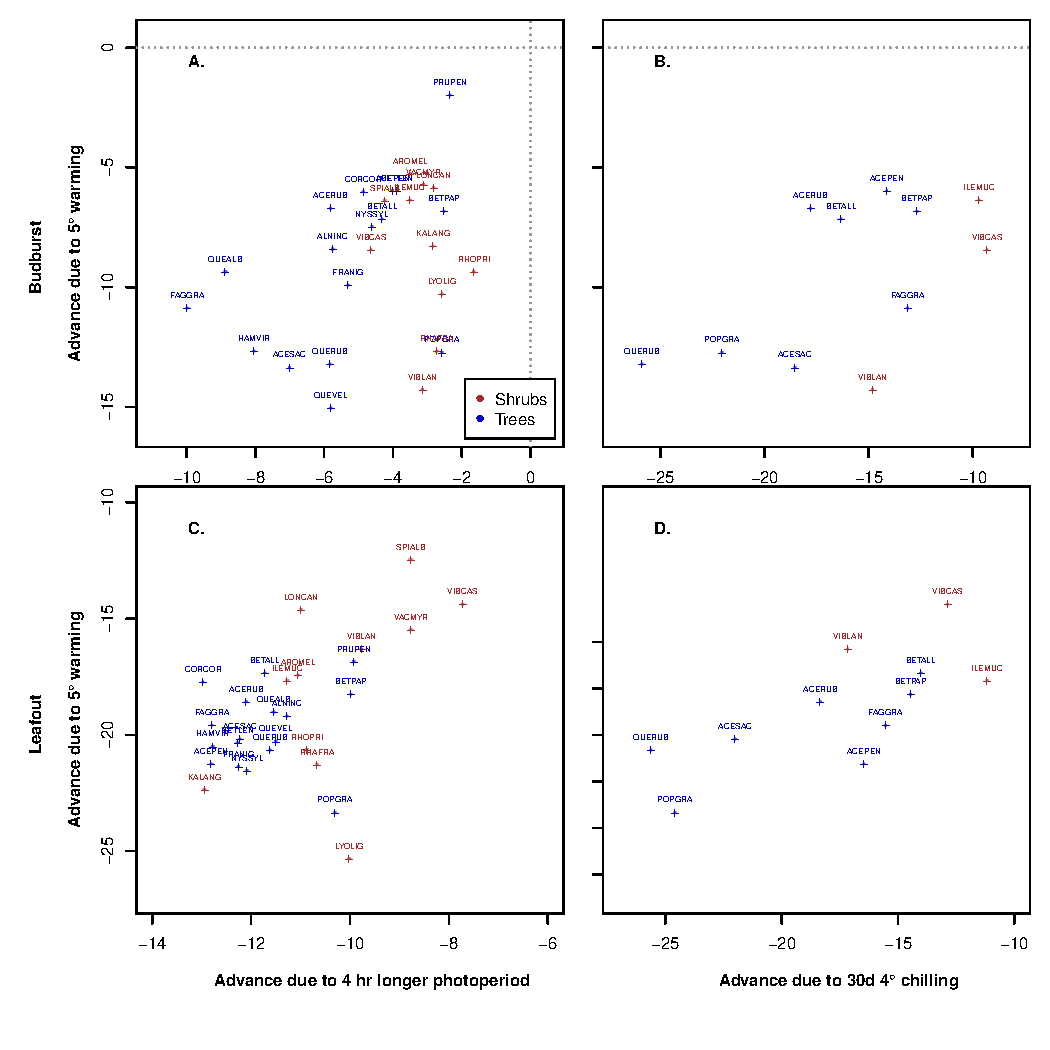
\includegraphics[scale=0.9]{Fig2_4panel}
\label{fig3}
\end{figure}

\end{document}}
